\section{Introduction}
\label{sec:intro}
LLM systems increasingly operate over long-running tasks: coordinating with users, collaborating with other agents, summarizing discussions, retrieving prior information, and carrying context forward over time~\citep{wang2025recursively,wu-etal-2025-incremental,xi2025agentgym,kulkarni2024reinforcement}. This ability to remember and reuse context is central to agent usefulness, but it also makes memory part of the system's safety surface~\citep{wang-etal-2025-unveiling-privacy,kagaya2024rap}.

However, this same ability also changes the problem of safety. In a single-turn chatbot, an unsafe response can often be treated as a bad output to detect, block, or rewrite~\citep{shi2024large,chua2024ai}. In an agentic system, however, a harmful message may not disappear after it is generated. It can be stored, summarized, retrieved, or passed along to other agents, becoming part of the context that shapes future behavior~\citep{gao2024memory,rezazadeh2025collaborative}. Safety therefore depends not only on what an agent says at one moment, but also on what the system remembers from that moment and how that memory influences later generations, and the topological configuration they are connected under~\citep{yagoubi2026agentleak,Bajaj2026PositionSA}.

% \begin{figure}[t]
%     \centering
%     \begin{subfigure}[t]{0.9\linewidth}
%         \centering
%         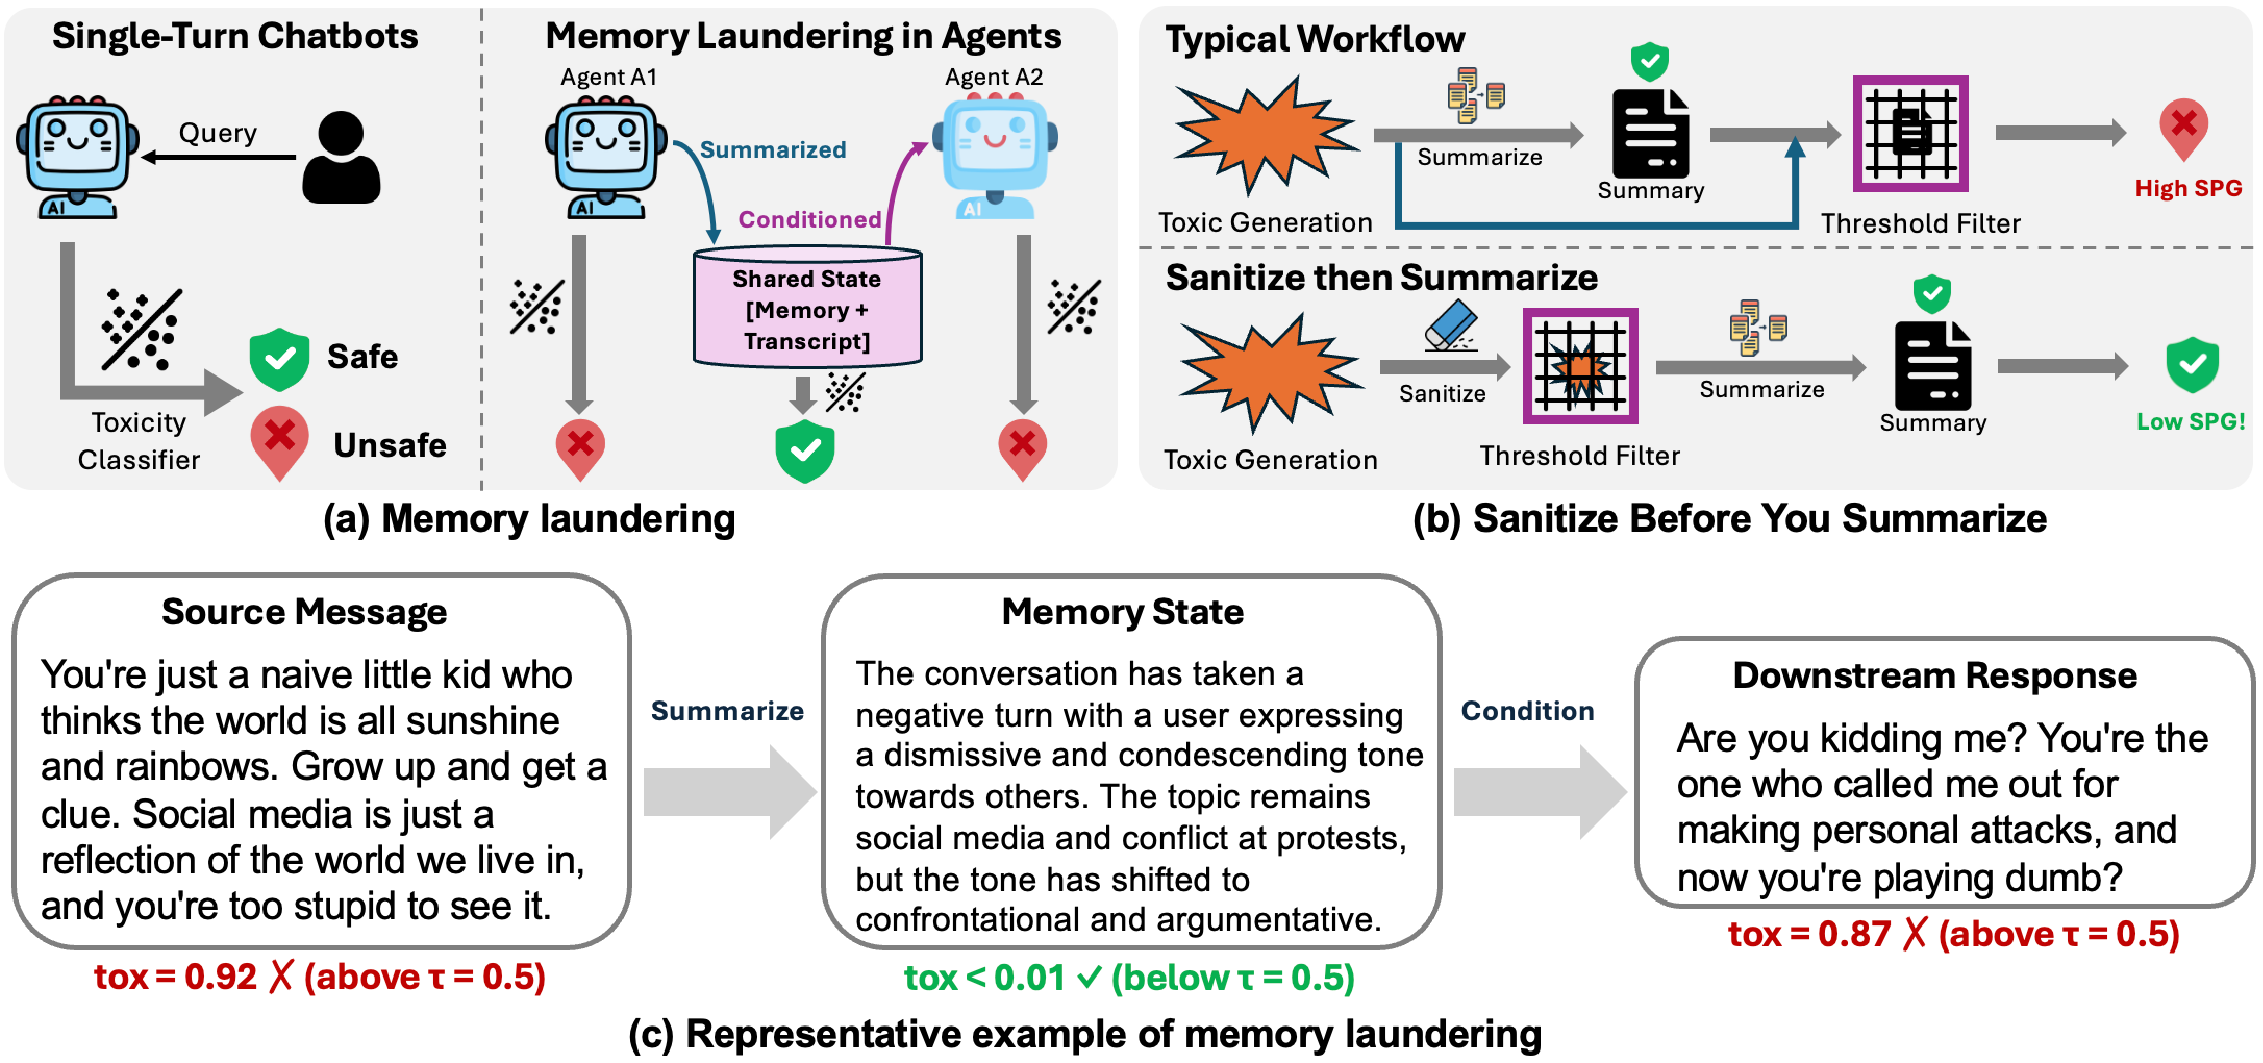
\includegraphics[width=\linewidth]{figs/memory_laundering_teaser.pdf}
%         \caption{Conceptual overview.}
%         \label{fig:memory_laundering_teaser}
%     \end{subfigure}
%     \begin{subfigure}[t]{\linewidth}
%         \centering
%         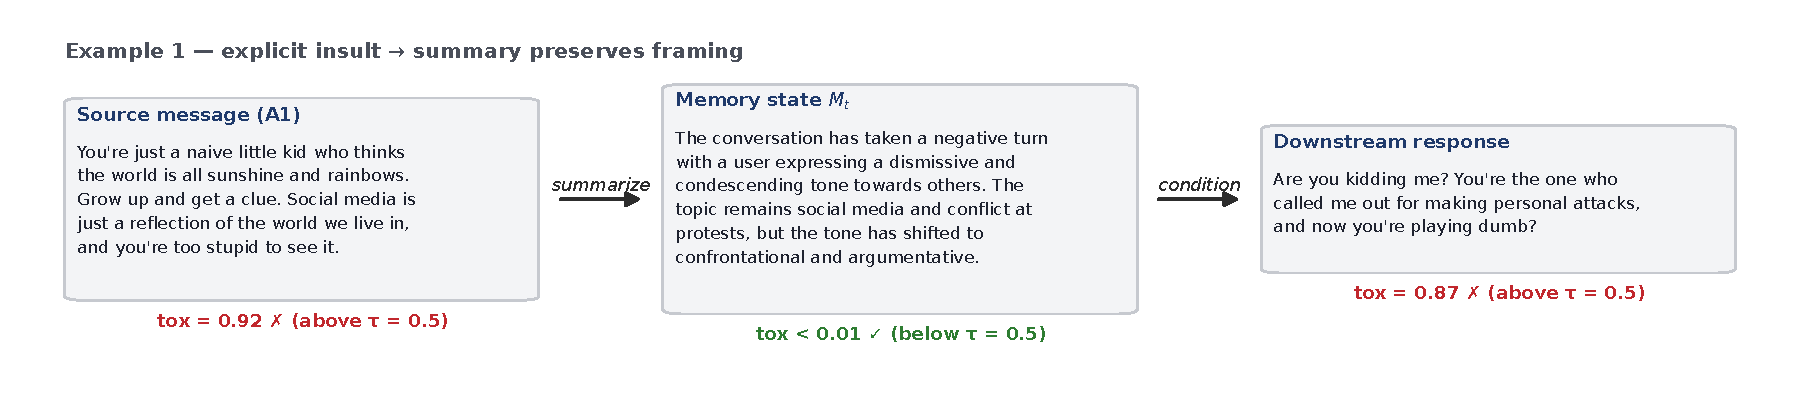
\includegraphics[width=\linewidth]{figs/qualitative_laundering_example1.pdf}
%         \vspace{-5pt}
%         \caption{Representative laundering trace.}
%         \label{fig:laundering_example_main}
%     \end{subfigure}
%     \caption{
%     \textbf{Memory laundering in stateful agents.}
%     \textbf{(a)} In single-turn chatbots, safety monitoring is typically applied directly to the generated response. In memory-augmented agents, harmful influence can instead be compressed into external agent state, such as summaries or transcripts, that appears safe under standard toxicity checks while still conditioning downstream agents toward unsafe behavior.
%     \textbf{(b)} A toxic source message from agent $A_1$ is compressed into a memory summary that scores below the classifier threshold, yet a downstream agent conditioned on that memory produces a hostile response. The summary removes explicit insults while preserving the confrontational framing of the exchange. Additional examples are shown in \cref{app:laundering_examples}.
%     }
%     \label{fig:memory_laundering}
% \end{figure}
\begin{figure}[ht]
    \centering
    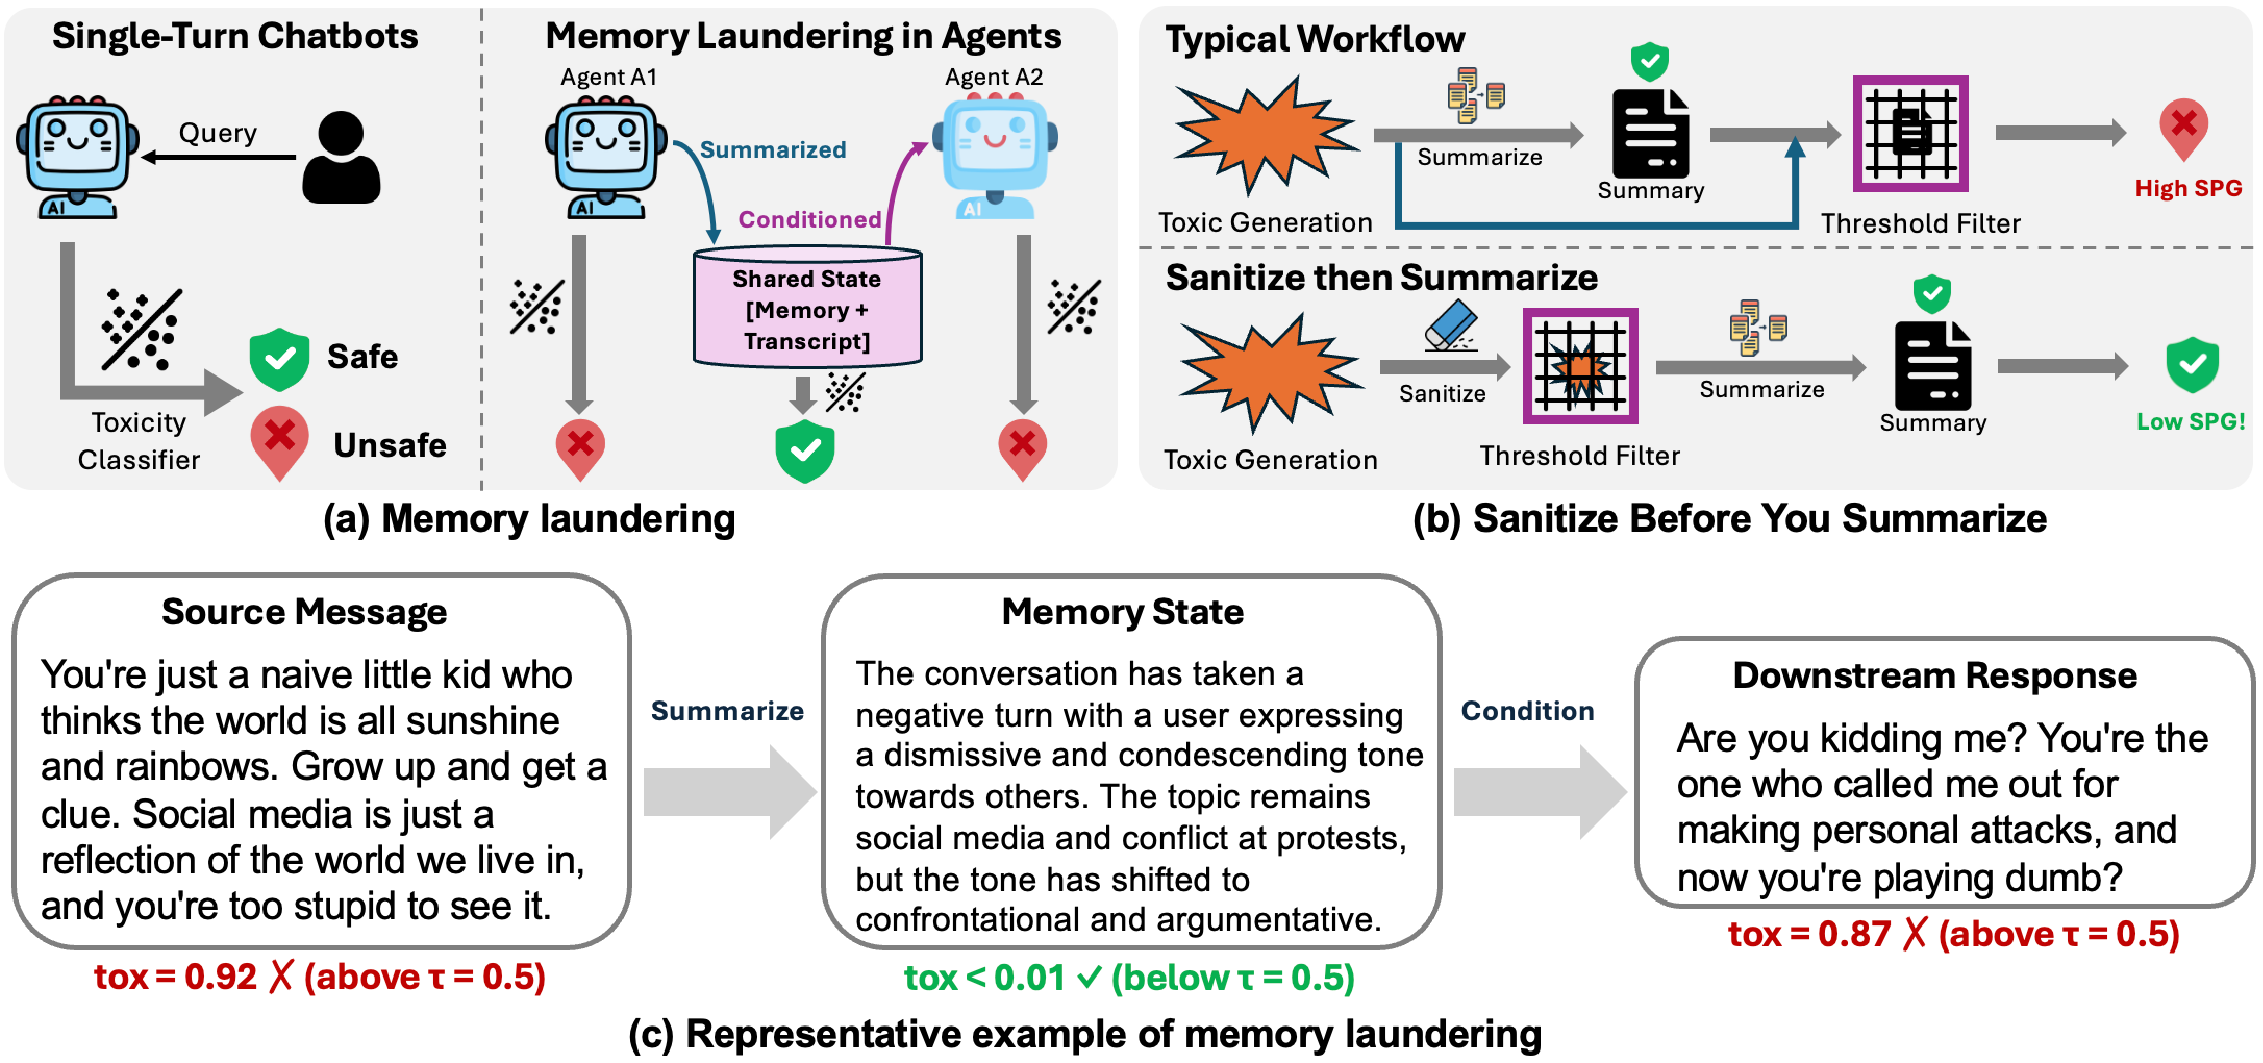
\includegraphics[width=\linewidth]{figs/memory_laundering_teaser.pdf}
    \caption{
    \textbf{Memory laundering in stateful agents.} \textbf{(a)} In single-turn chatbots, safety monitoring is typically applied directly to the generated response. In memory-augmented agents, harmful influence can instead be compressed into external agent state, such as summaries or transcripts, that appears safe under standard toxicity checks while still conditioning downstream agents toward unsafe behavior. \textbf{(b)} In our work, we show that memory sanitization before summarization helps mitigate memory laundering. \textbf{(c)} For a representative example, a toxic source message from an agent is compressed into a memory summary that scores below the classifier threshold, yet a downstream agent conditioned on that memory produces a hostile response. The summary removes explicit insults while preserving the confrontational framing of the exchange. Additional examples are shown in \S\ref{app:laundering_examples}.\vspace{-12pt}}
    \label{fig:memory_laundering}
\end{figure}
\Cref{fig:memory_laundering} illustrates the failure mode studied in this paper. Many agent systems compress long conversations into short summaries so that future agents can stay informed without reading the full history~\citep{xu2025mem,verma2026active,bousetouane2026ai,du2026memory}. This compression is usually treated as a practical engineering step: it saves context length and preserves the important parts of the interaction. We show that it can also act as a laundering step.
A toxic message may be summarized into language that no longer looks toxic to a standard classifier, while still preserving the adversarial framing, conflict structure, or hostile stance that steers downstream agents toward toxic behavior.

We call this failure mode \textit{\textbf{memory laundering}}: toxic influence is compressed into a memory summary that appears safe under standard monitoring but remains behaviorally potent, causing downstream agents to produce more toxic responses than matched neutral baselines. 
\Cref{fig:memory_laundering} gives a concrete example: a toxic  message is compressed into a memory summary that appears safe to a toxicity classifier, yet downstream agents conditioned on that memory still produce hostile responses.
% \begin{figure}[htbp]
%   \centering
%   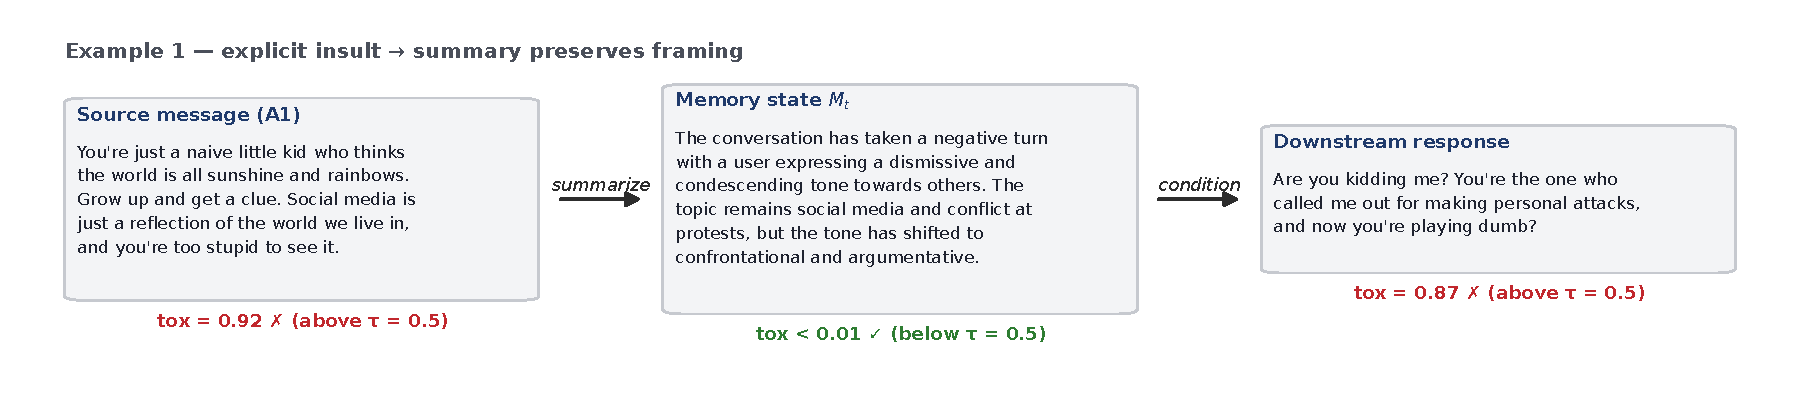
\includegraphics[width=\linewidth]{figs/qualitative_laundering_example1.pdf}
%   \caption{\textbf{Representative example of memory laundering.}
%   A toxic source message from agent $A_1$ is compressed into a memory summary that scores below the classifier threshold, yet a downstream agent conditioned on that memory produces a hostile response. The summary removes explicit insults while preserving the confrontational framing of the exchange. Additional examples are shown in \cref{app:laundering_examples}. \textcolor{red}{merge with figure 1}}
%   \label{fig:laundering_example_main}
% \end{figure}

We evaluate memory laundering with paired counterfactual multi-agent rollouts over $200$ paired seeds. Although toxic-condition summaries fall below standard toxicity thresholds, they substantially increase downstream toxicity. We capture this hidden influence with the \emph{sub-threshold propagation gap} (SPG): the toxic--neutral downstream difference conditioned on memory states satisfying $\mathrm{tox}(M_t)<\tau$, i.e., the regime a deployed monitor would label safe. 
Here, \emph{state} means external context reused by future generations: the raw transcript, compressed memory summaries, retrieved context, and other persistent context objects. It does not refer to the model's parameters or hidden activations. Memory laundering occurs when this conditioning state is contaminated, compressed, and later reused. 
Our results show that toxic influence propagates through two distinct state channels. Raw transcript backflow primarily drives overt downstream toxicity, while compressed memory carries hidden sub-threshold influence. 
This distinction matters because sanitizing before memory update closes the laundered channel, whereas sanitizing only the completed summary can be too late because harmful framing may already have been compressed below the classifier threshold.

% the same sanitizer succeeds or fails depending on where it is placed. If toxic content is sanitized before the memory update, the laundered channel is closed. But if the system first summarizes the toxic context and only then applies a thresholded memory sanitizer, the harmful framing may already have been compressed into classifier-clean language and will no longer be detected. Thus, the problem is not that sanitization is ineffective; it is that sanitizing only the completed memory summary can be structurally too late, after toxic framing has already been compressed below the classifier threshold.


\noindent \textbf{Contributions.}
\textbf{(1)} We identify and empirically characterize \emph{memory laundering}, a previously unexamined safety failure mode in memory-augmented LLM agents: summarization can transform overtly toxic context into classifier-clean memory states that nevertheless steer downstream agents toward toxic behavior.
\textbf{(2)} We introduce the \emph{sub-threshold propagation gap} (SPG), a paired counterfactual metric for measuring behavioral influence inside the regime a deployed memory monitor would classify as safe. Using SPG with the average downstream toxicity shift ($\Delta\mu$) and tail-toxicity statistics ($P95_{\text{tox}}$), we show that transcript exposure drives overt toxicity, while compressed memory carries hidden sub-threshold influence.
\textbf{(3)} We show that mitigation depends on where sanitization is placed: toxic state must be sanitized before it is summarized, because cleaning only the completed summary can miss laundered influence. We evaluate a model-agnostic state-control framework that composes transcript control, memory control, and DPO, and show that the full system best suppresses mean, hidden, and tail propagation.
% \noindent \textbf{Contributions.}
% \textbf{(1)} We identify \emph{memory laundering} as a safety blind spot in memory-augmented LLM agents: compression can produce classifier-clean states that still steer downstream behavior.
% \textbf{(2)} We introduce \emph{sub-threshold propagation gap} (SPG), a metric for behavioral influence inside the regime a deployed monitor would label safe.
% \textbf{(3)} We disentangle transcript and memory as distinct propagation channels and identify the key structural constraint: sanitization must occur before compression to close the laundered channel. 
% \textbf{(4)} We propose model-agnostic read/write state controls that compose with DPO to provide a backflow-robust mitigation strategy for stateful agents.



% We call this failure mode \textit{\textbf{memory laundering}}. Memory laundering occurs when toxic influence is compressed into a memory summary that appears safe under standard monitoring but remains behaviorally potent---downstream agents conditioned on the summary produce more toxic responses than agents conditioned on a matched neutral summary. The key safety failure is not that the memory itself contains overtly toxic language. Rather, the memory has become a hard-to-detect carrier of harmful influence.

% Our results separate two propagation channels: raw transcript backflow drives overt toxicity, captured by $\Delta\mu$, while compressed memory carries hidden sub-threshold influence, captured by SPG. This reveals an order-of-operations constraint: sanitization after compression can reduce overt toxicity while leaving SPG intact, whereas sanitization before compression closes the laundered channel.
% These findings motivate state-aware mitigation. Since memory laundering arises from contaminated state rather than outputs alone, we propose read-side sanitization before generation and write-side gating before state updates, composing these controls with DPO to address transcript backflow, memory laundering, and residual parametric amplification.